\section{Introduction}
\label{sec:intro}

隨著線上外送平台如 Foodpanda 和 UberEat 的迅速發展,餐飲產業的數位化轉型逐漸加快。這些平台不僅縮短了顧客與餐廳之間的距離,還利用大數據分析技術來優化用戶體驗並提升平台的營收效率。在此背景下,餐廳推薦系統扮演了關鍵角色。它通過分析顧客的歷史消費行為、偏好,以及當前的流行趨勢,實現個性化推薦,進一步提高了推薦的準確性和顧客的滿意度。
傳統的推薦系統方法,如基於內容的過濾 (content-based filtering) 和協同過濾 (collaborative filtering),能夠在一定程度上提供有效的推薦,仍難以捕捉到顧客與餐廳之間更深層的關聯結構。隨著圖神經網路 (Graph Neural Networks, GNN) 的應用擴展,人們發現可以將顧客與餐廳之間的互動關係表示為圖結構,以便從更高層次上捕捉其複雜的互動模式。這種關聯結構可以使用二分圖 (bipartite graph) 來表示。

\begin{figure}[tbh]
    \centering
    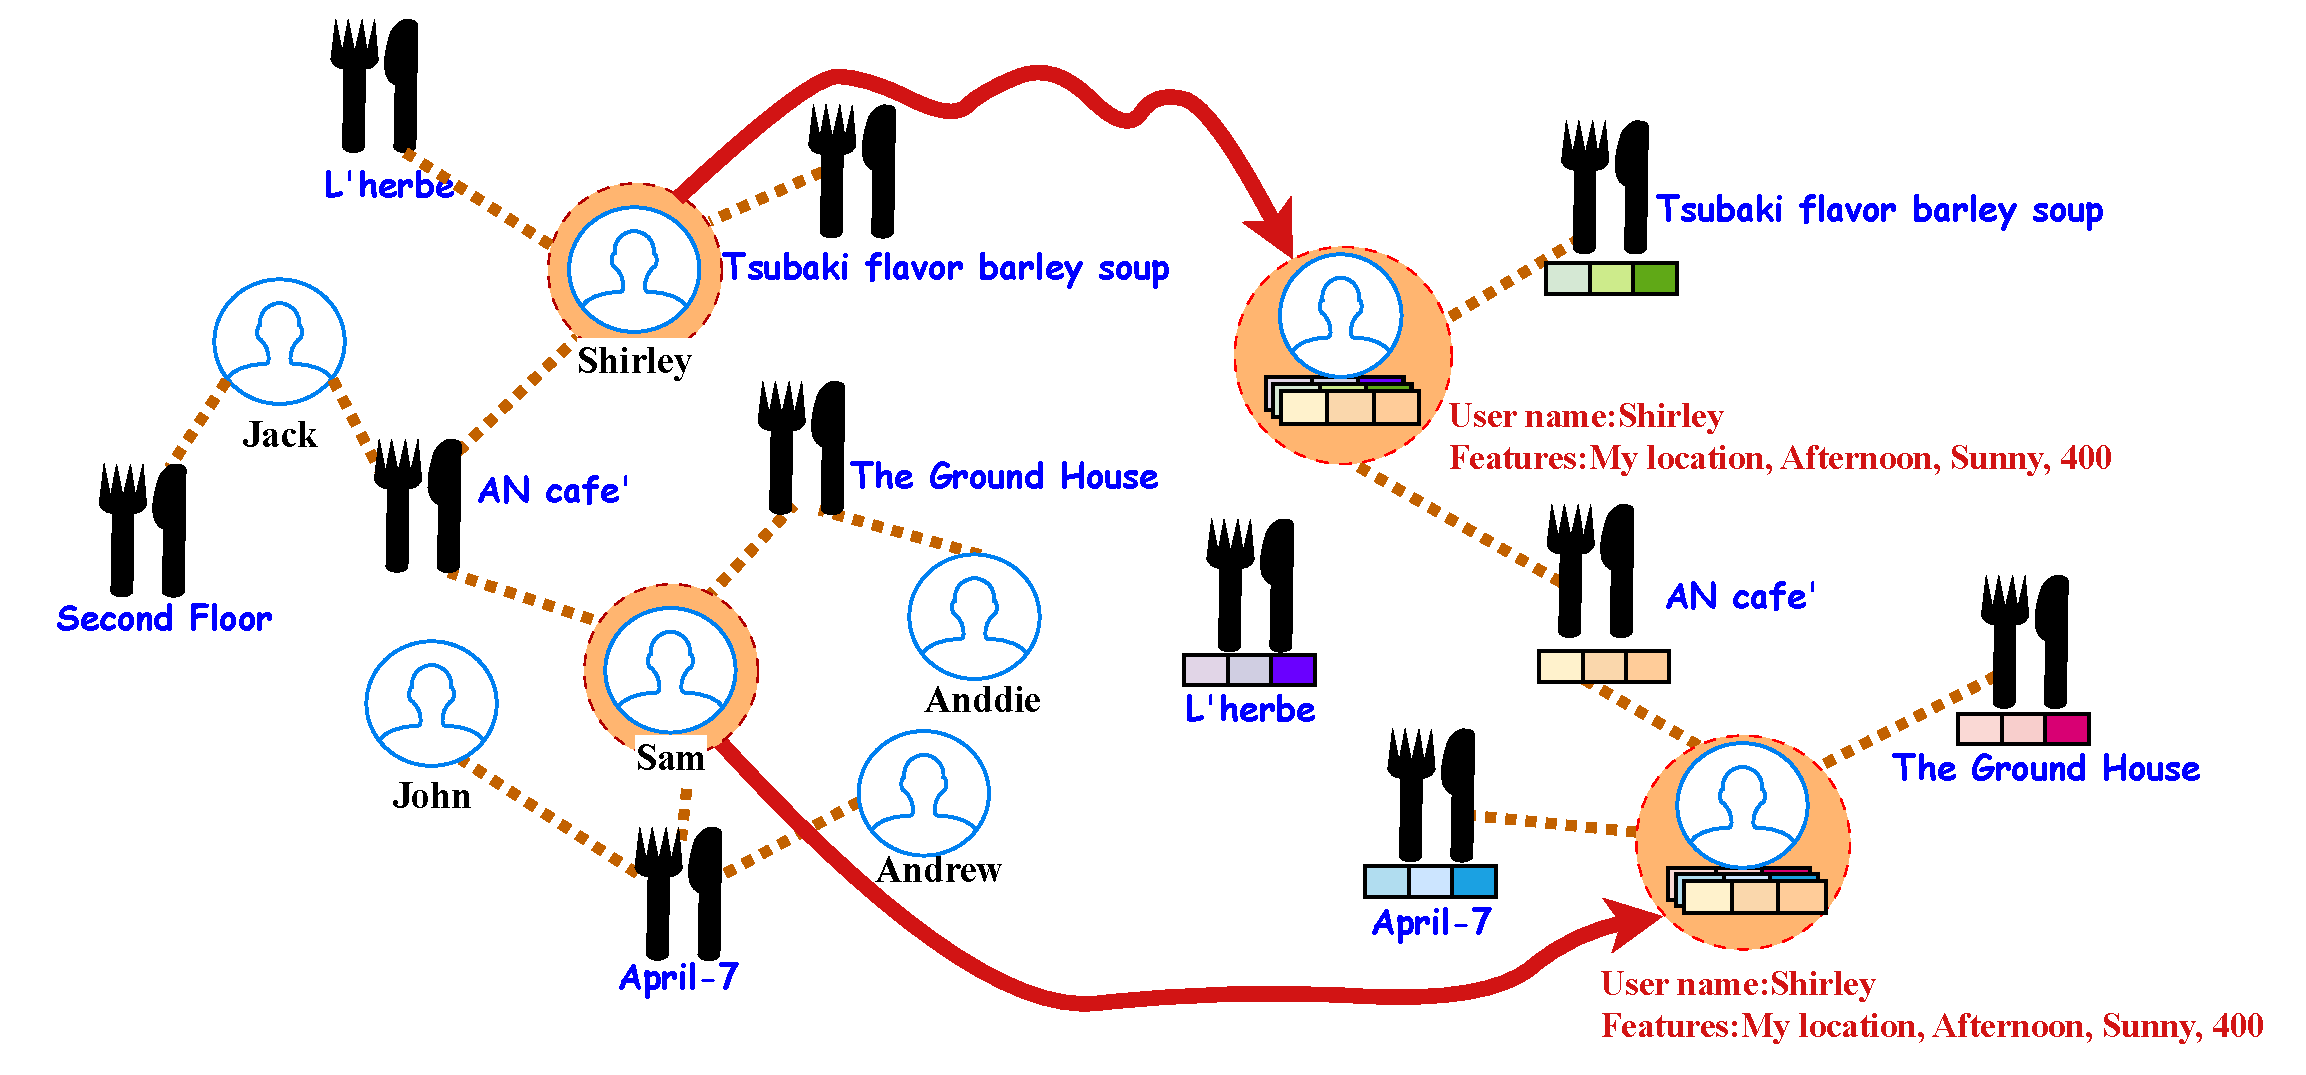
\includegraphics[width=0.5\textwidth]{img/bipartite_graph.pdf}
    \caption{推薦系統中的二分圖示意~\cite{bipratite_fig}}
    \label{fig-bipartite}
    \vspace{-0.35cm}
\end{figure}

如圖~\ref{fig-bipartite} 所示,節點可以分為兩類:使用者節點和餐廳節點,兩者節點類型的不同使得該圖同時為異質圖 (attributed heterogeneous graph)。本研究使用 Zhang 等人提出的 NIE-GCN 方法~\cite{NIE-GCN},從該資料集的二分異質圖中提取出更深層的連結信息,以預測顧客節點最感興趣的前 $k$ 個餐廳節點,進一步優化推薦精度。最終以歸一化折扣累積增益 (Normalized Discounted Cumulative Gain, NDCG) 和召回率 (Recall) 作為評估推薦系統表現的指標,為平台提供精確的推薦評估依據。
\begin{figure}[tbh]
    \centering
    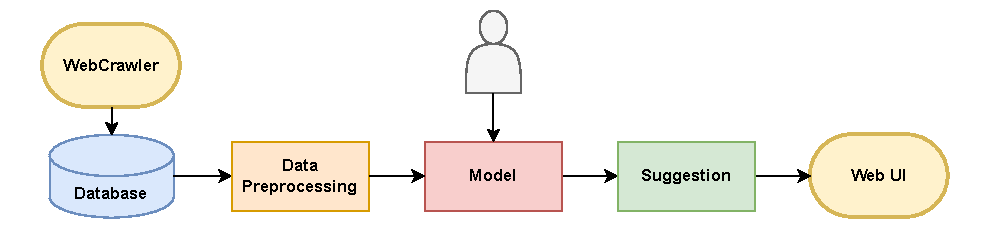
\includegraphics[width=0.5\textwidth]{img/flowg2.pdf}
    \caption{推薦系統架構圖}
    \label{fig-flowchart}
\end{figure}
本研究的架構如圖~\ref{fig-flowchart} 所示。首先,透過爬蟲技術從 Foodpanda 和 Google Maps 上獲取每個餐廳的資訊,並將這些資料儲存到資料庫中。接著進行基本的資料前處理,為模型的輸入做好準備。在使用者節點上,所包含的資訊如表~\ref{node-conetent} 所列。這些資訊經處理後會被輸入到模型中,最終生成推薦結果,並透過 Web UI 進行呈現。
\begin{table}[htbp]
    \centering
    \renewcommand{\arraystretch}{1.15}
    \setlength{\tabcolsep}{7.5pt}
    \begin{tabular}{|c|c|}
    \hline
    \textbf{節點類型} & \textbf{節點內容} \\ \hline
    使用者 & 當下位置、使用時間、天氣、預算 \\ \hline
    推薦餐廳 & 餐廳名稱、價位、評分、評論 \\ \hline
    \end{tabular}
    \caption{使用者與推薦餐廳的節點資訊}
    \label{node-conetent}
\end{table}
透過這些節點資訊,本研究可以針對不同使用情境生成個性化推薦,讓系統在多維度考量下更精確地滿足使用者需求。





    